\documentclass[12pt]{article}
\usepackage{fullpage,enumitem,amsmath,amssymb,graphicx,hyperref,footmisc}
\usepackage[margin=1in]{geometry} 
\renewcommand{\thefootnote}{\fnsymbol{footnote}}
\begin{document}

\begin{center}
{\Large CS221 Fall 2016 Project Final Report: Scrabble AI}

\begin{tabular}{rl}
  Authors: & Colleen Josephson $\{$cajoseph$\}$ and Rebecca Greene $\{$greenest$\}$\\
\end{tabular}
\end{center}


\section*{Introduction}
The goal of our project is to build an AI that plays Scrabble, a
popular crossword board game in which players build words on a 15x15
board using tiles representing letters. Different letters have
different values, and the number of points a player receives for
forming a word is equal to the sum of the values of the tiles in the
word, with multipliers depending on location on the board. There are a
fixed set of tiles in the game, and at any point in the game, each
player has access to at most 7 letter of these in their 'rack'.  When
tiles are placed on the board they are replaced with ones drawn at
random from a bag. If the players uses all 7 tiles this is called a
'bingo' and the move receives a 50pt bonus, which can be about 1/8 of
the total points in a tournament game.

Since each player can make no direct observations of the other
player's rack, Scrabble can be considered a stochastic partially
observable game [Russel and Norvig, 2003]. Thus it is very different
from many games like Othello, chess, or Go in which each player has
complete knowledge of the state of the game at any point. In addition,
the incredible number of possible moves renders typical decision-tree
models to be all but impossible.

In the following sections we will discuss the background and prior
work, our approach to solving the problem, our experimental
infrastructure, and an analysis of the results.\\

\section*{Background and Prior Work}

A number of previous Scrabble AIs have been developed, starting with a
Scrabble/crossword playing program developed by C. Sharpiro at the
University of New York at Buffalo in 1982, and continuing today with
Scrabble/crossword AIs like Quackle and Elise.

One of the most important publications in the history of Scrabble AIs
was a paper by Andrew Appel and Guy Jacobson published in 1988 on 'The
World's Fastest Scrabble Program'. It in, Appel and Jacobson describe
the move generation algorithm that has since been used by all major
Scrabble AIs. They convert the lexicon into a data structure called a
'directed acyclic word-graph' or 'dawg', that greatly expedites the
search for valid moves. We use a simplified version of this this
algorithm, substituting dawgs for tries, which will be explained in
greater detail below.

The most famous Scrabble AI was a program called 'Maven' that was
developed by Brian Sheppard in 2002, which was the first Scrabble AI
to beat human champion players.  Maven divides the game Scrabble game
into three subcategories-- regular game play, the pre-end game, and
the end-game. The 'end game' is the period after which all letters in
the bag have been used. At this point the 'end game' is the period
after which all letters in the bag have been used. At this point the
game becomes completely observable, and a B* search on a game tree can
be used to optimize agent game play. We based a lot of our
implementation on the regular game play strategies used by Maven, but
ignored the pre-end game and end-game aspects of the game, as we were
limited on time, and found the problem a less interesting
pursuit. Maven is the AI currently used in official Hasbro Scrabble
games.

The current champion of the Scrabble AIs is Quackle, developed by 5
researchers at MIT. Quackle uses a strategy that is very similar to
Maven's. Quackle is the current measuring stick against which all
other Scrabble AIs are compared, and we analyze our AI's performance
against Quackle later in the paper.

\section*{Approach}
Extensive vocabulary alone is not sufficient for a competitive
Scrabble player. If a player optimizes for the best score on every
turn they tend to retain tiles that are more difficult to use in play,
leading to future racks that will produce a lower score. The best
Scrabble players try to maintain their rack in a way that will be
conducive to future high-scoring plays.

Computers can be preprogrammed with the entire permissible dictionary,
since that dictionary is about 200,000 words long, and the 7 letters
on the rack can be combined with those on the board in tens of
thousands of different permutations, the search for possible moves
becomes a nontrivial undertaking. Most Scrabble AIs give themselves a
time limit to ensure reasonable progress of play.

Once a list of possible moves has been generated, the AI needs to
select the best move as a weighted decision of the score that the move
would generate, the opportunities it would provide of the other
player, and the effect it would have on the future rack.

Scrabble AIs face the following challenges:
\begin{enumerate}
  \item \textbf{Move generation:} create a list of possible moves from
    the state of the board, the letters in the rack, and the allowable
    words in the dictionary. This is a nontrivial search problem.
    
  \item \textbf{Rack maintenance:} balance the tradeoff between getting
    the maximal score for a given turn with maintaining a rack that
    will be useful for future turns, which usually involves a weighted
    sum acquired with machine learning plus a number of Monte Carlo
    simulations.
    
  \item \textbf{Adversarial gameplay:} avoid creating opportunities
    for the other player to place high scoring words 
\end{enumerate}

Once the bag has been emptied (all tiles are either on the board or in
one of the racks), the game switches to being one with a completely
known state. At this point evaluation techniques like minimax become
useful to maximize score. This is commonly referred to as
\emph{endgame strategy}, and typically only state-of-the-art AIs go
into this level of detail.

\subsection*{Model and Algorithms}
\subsubsection*{Move Generation}
To help solve the search problem, we're using an algorithm created in
the 1980s by Andrew Appel and Guy Jacobson. This algorithm remains the
backbone of most competitive Scrabble AIs today. Appel and
Jacobson propose restructuring the Scrabble lexicon from a list of
words into a trie or prefix tree, where each node is a partial word,
the children of a node are words or partial words that can be created
using that node (see Fig. 1). All terminal leaves of the trie are
words, as are some interim nodes (e.g 'dog' vs. 'dogs'), and the value
of a node is a boolean indicating whether the sting is a full word in
the dictionary.


\begin{center}

From Appel-Jacobsen '86\\
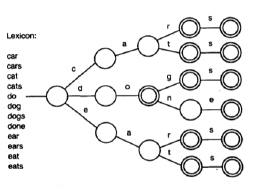
\includegraphics[scale=0.6]{../images/trie}\\
Figure 1: An Example of a Trie \\
\end{center}

%% We found the pytrie library rather helpful for implimenting this
%% algorithm, as it's CharTrie object was designed for implimentations
%% such as this, where the children of a node are held in a dictionary
%% that is indexed by letter (ex. startNode.children = {'c': <node
%%   object>, 'd': <node object>, 'e': <node object>). The maximim number
%%   of edges from a node is 26. Appel and Jacobson actually further
%%   reduce this to save on memory by combining nodes, but since we are
%%   now almost 30 years in the future, memory is less of a concern, so
%%   we decided to leave our dictionary as a trie.
  
To search for moves on the board, the algorithm examines all
\emph{anchors}, where an anchor is the space to the left (or above) an
existing letter (for horizontal plays), or the space above an existing
letter (see Fig. 2). Since a move in Scrabble must attach to an
existing word (excepting the first move), this greatly reduces the
15x15 search space. After each new move on the board, the AI should
update its list of anchor squares.

\begin{center}
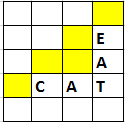
\includegraphics{../images/anchorexample}\\
Figure 2: An Example of Anchor Squares
\end{center}

Before a potential move is added to the list of generated moves, it
needs to be \emph{crosschecked} to ensure that new strings formed in
the orthogonal dimension also exist in the dictionary. For example, in
Figure 3, when placing DOG underneath CATS, AD and TO are real words,
but the vertical SG would fail a crosscheck.  Since the crosscheck
results for a given tile remain static unless the tiles adjacent to it
change, the checks only need only be updated once per move, and only for the
squares immediately adjacent to newly placed tiles.

The heart of the algorithm is a backtracking search with constraints
that the final result must be a valid word (enforced by the structure
of the trie itself), all crosschecks pass, and the new letters placed
on the board come from the player's rack. The search algorithm has two
recursive parts: ExtendLeft and ExtendRight. Below is pseudocode for
the backtracking algorithm to place a horizontal word:\\

\quad ExtendRight (PartialWord, node N, square):

\quad\quad if square is not empty:

\quad\quad\quad if the letter l in square is an edge of N (PartialWord + l is a node):

\quad\quad\quad\quad ExtendRight(PartialWord + l, N.children[l], nextSquare)

\quad\quad else:

\quad\quad\quad if PartialWord is a word: LegalMoves.append(PartialWord)

\quad\quad\quad for each letter l that is in rack and an edge out of N

\quad\quad\quad\quad\quad\quad\quad\quad and in the cross-check set of square:

\quad\quad\quad\quad\quad remove l from the rack

\quad\quad\quad\quad\quad ExtendRight(PartialWord + l, N.children[l], nextSquare)

\quad\quad\quad\quad\quad put tile l back into the rack\\


ExtendLeft places tiles to the left of the anchor point and then calls
ExtendRight. 'Limit' is the number of blank tiles
between the current anchor point and the preceding anchorpoint (or the end of the board), capped at the rack size of 7.\\

\quad ExtendLeft(PartialWord, node N, square, limit):

\quad\quad ExtendRight(PartialWord, N, square)

\quad\quad if limit $>$ 0: 

\quad\quad\quad for each letter l in rack that is an edge of N: 

\quad\quad\quad\quad remove l from the rack

\quad\quad\quad\quad ExtendLeft(l+PartialWord, N' =
N.children[l], nextSquare, limit -1)

\quad\quad\quad\quad put tile l back into the rack\\
			
To generate a list of all legal moves for a given board, call
LeftExtend("", root node, anchorSquare, Limit) on all anchors. See
Figures 1 and 2 in 'Examples and Preliminary Data'

%Based off appel-jacobsen is move generation algo, we will do a
%backtracking search on a trie where the letters are edges and nodes
%are partial words/words (leaf nodes are words). The maxmum number of
%edges from a node is 26. The trie is pre-computed from the dictionary.

%The trie itself enforces the constraint of each tile-placement being
%the substring of a word in the dictionary. The backtracking search
%will enforce the other constraints, namely:
%-selected letters must come from the player's tile set
%-word must not form a non-word with another part of the board
%-word must fit on the board

%From there, we will generate all possible moves (or some randomized
%subset of them, if this is far too time-consuming) and choose maximal
%weight move, where the weight is the standard Scrabble score
%function. Some Scrabble AIs have additional heuristics in the score,
%such as weighting words based on how they impact the tile rack. We
%stuck with the simple scording function for the first pass, but may
%conisder additional heuristics for the final result.

\subsubsection*{Rack Maintenance and Adversarial Gameplay}
The next step of the problem is to try to decide which of the legal
moves is best, given consideration of score, maintaining a reasonable
rack, and not giving any advantages to the opponent. This is best done
through a combination of Monte Carlo simulation and linear predictors
with learned weights.

The raw score of a move is as a function of tile values and
multipliers on the board, plus any resulting multi-word bonuses or
bingos. This is simple to compute, but also a simplified view of the
situation. A better metric is the agent/opponent point differential
obtained as the result of a move, which is the result of the raw score
of the move and also the opportunities it proves the opposing
player. This differential is best computed through simulation. For
each of the top raw-scoring moves, the AI runs a number of Monte Carlo
simulations playing against itself with probable opponent racks. Since
the turnover rate of racks is so high, and the computation required
per move is rather extensive, most competitive AIs run their models
with a search depth $\geq 3$. Our preliminary algorithm does not
implement this, but we would like to add it for the final product.

Many Scrabble AIs don't try to make any assumptions about the opposing
player's rack, and just assign the opponent random unseen letters when
running simulations. However, it is possible to use Bayes' algorithm
to make a probabilistic model of the tiles a player had on their rack
at the start of a turn given the move they made during that turn.%% This
%% is equivalent to having a model of many of the tiles the opposing
%% player will have on their rack for the next turn (the rest are
%% filled in at random from the letter bag).
For instance, if the opposing player used the letters 'C, T' to attach
to an A and make "CAT", it is unlikely that they left an S on their
rack, because otherwise they would have played "C,T,S" to make "CATS",
which is a higher scoring word. More formally $P(leave | play) =
\frac{P(play | leave)P(leave)}{P(play)}$, where P(leave) is the
probability that certain tiles were left on the rack. When an AI's
Monte Carlo simulations draw from this probability space rather a
random assignment, the algorithm has better performance on a level
that is statistically significant(Richards and Amir, 2007).

	
Now that the scores have been computed by simulation, they are weighed
along with heuristics for rack maintenance to select the best move to
use. The features extracted for this purpose are:

\begin{enumerate}
  \item whether or not a given tile is present in the rack
  \item duplicated tiles, e.g. in the rack AABCDEF 'AA' would be a double
  \item triples of a tile(CCC) for different letters
  \item balance of vowels and constants (which has been proven to be
    an important factor in weight maintenance
  \item whether or not 'Q' has a corresponding 'U' in the rack at the same time
\end{enumerate}

The weights for these features are learned by initially setting them
all to zero, and having the AI play itself, running a stochastic
gradient ascent since we want to \emph{maximize} the score
differential. Consequently the loss function we use is $\mathbf{w}
\cdot \phi(A) - \mathbf{w}\cdot \phi(B)$. The SGA is implemented in
sga.py.

\section*{Experimental Infrastructure}
The two primary ways to test AIs are against humans or against other
AIs. A common benchmark is whether or not an AI can beat a human world
champion.

We did test our game against people, but collecting that data is time
consuming and logistically challenging. To generate our data we played
our AI against Quackle. We also played variants of our AI against
itself. The variants we created are:

\begin{itemize}
\item \textbf{vanilla:} selects max scoring move from Appel-Jacobsen
  move generation algorithm
\item \textbf{rack heuristic:} selects N moves with the top raw scores
  and creates a feature vector from the raw score and features
  extracted from the remaining rack, and applies a weight vector
  learned via 100-iteration stochastic gradient run. The move with the
  max weighted score is returned
\item \textbf{Monte Carlo:} selects the top N scoring moves and
  simulates M different depth D future plays, and returns the score
  differentials for each move weighted by the probability of the
  opponent being able to make that move. For our results, we used N=3,
  M=15 and D=2.
\item \textbf{Monte Carlo + rack heuristic:} includes the Monte Carlo
  score in the feature vector and applies a different weight vector;
  the move with the top weighted score is returned
\end{itemize}

\subsection*{Quackle vs CS221 Mode}
Playing against Quackle in an automated manner proved to be a
reasonably challenging task, as our code is in Python while Quackle
was written in C++. To avoid re-implementing our AI in C++, we used a
file-based system for interprocess communication. We modified the test
system for Quackle in quackle/test/testharness.cpp to interface with
out AI via reading and writing moves to files. We created one main
method, \textbf{selfPlayCS221Game}().

For the Python half, we wrote 'autorun.py', which starts the Quackle
test harness and reads and writes to the shared files until the
specified number of games has been played. The scores are stored in a
dictionary, which is printed out at the end so the data can be
processed in Scrabble/images/plot.py.

This was the most challenging part of our infrastructure to set up, but
as a result we are able to see how our AI compares to world-class AI.

\subsection*{Self Play Mode}
Playing our AI against itself is significantly more simple, and also
provides good data on how much the different variants improves
gameplay. Self-play mode is in selfrun.py, and does not require any
file IO.

\subsection*{Human Mode}

For testing various aspects of gameplay and to see how well the AI
performed against average-ability humans, we created a human vs AI
mode in run.py. Since human-generated data is time-consuming to
collect, and neither the authors nor their friends describe themselves
as skilled Scrabble players, we do not collect any statistics from
human mode.

\section*{Results and Analysis}
Overall, we are able to beat Quackle 11-13\% of the time with an
average score in the 280's. Since this is against a world class AI, we
are quite pleased with the results. Figures 1-4 show the \emph{score
  differential} between Quackle and our AI. The lower the
differential, the better. For example, a differential of 20 means that
Quackle won that game by 20 points.

Table 1 outlines additional statistics, such as the average scores of
each AI, the average score differential, the number of games we lose
by 2x points or more, and the maximum score ratio (a ratio of 1.5
means we scored 1.5 times as many points as Quackle for that game).
Entries in Tables 1 and 2 marked with \textbf{*} were shorter runs due
to time constraints. Table 1's MC+RH was 35 runs, and Table 2's MC and
MC+RH were 80 and 53 runs respectively. Furthermore, the MC+RC weight
vector was only run for 50 iterations instead of 100.

\begin{table}[h!]
  \centering
  \begin{tabular}{c|l|l|l|l|l|l}
    \textbf{} & \textbf{win rate} & \textbf{mean} & \textbf{opp mean} & \textbf{mean delta} &  \textbf{2x loss rate} & \textbf{max win ratio} \\\hline
  \textbf{vanilla}   & 11\% & 284.68 & 407.43 & 122.75 & 13\% & 1.358\\
  \textbf{RH}        & 13\% & 288.07 & 410.0  & 121.93 & 11\% & 2.131\\
  \textbf{MC}        & 13\% & 283.3  & 401.95 & 118.65 & 14\% & 1.42 \\
  \textbf{MC w/ RH*} & 5\%  & 285.38 & 412.22 & 126.83 & 13\% & 2.34 \\
\end{tabular}
  \caption{Statistics of our AI variants against Quackle's Speedy
    Player. \emph{Mean delta} is the average difference between
    opponent and our score, \emph{2x loss rate} is the rate at which
    the opponent scores 2x or higher, and \emph{max win ratio} is the
    max ratio of our score to opponent's.}
\end{table}

\begin{figure}[h!]
  \minipage{0.5\textwidth}
    \centering
  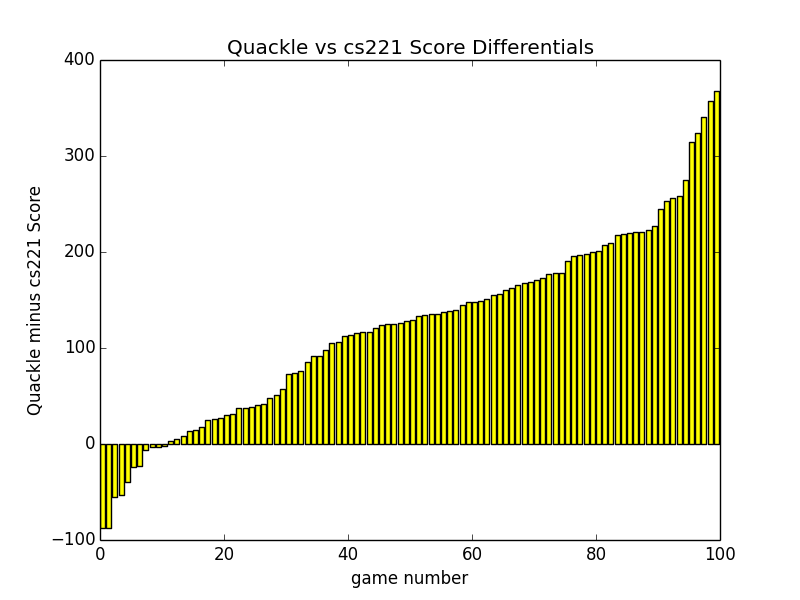
\includegraphics[scale=0.4]{../images/quacklegame_vanilla_100}
  \caption{\footnotesize{Quackle vs CS221 Vanilla}}
  \endminipage
  \minipage{0.5\textwidth}
      \centering
  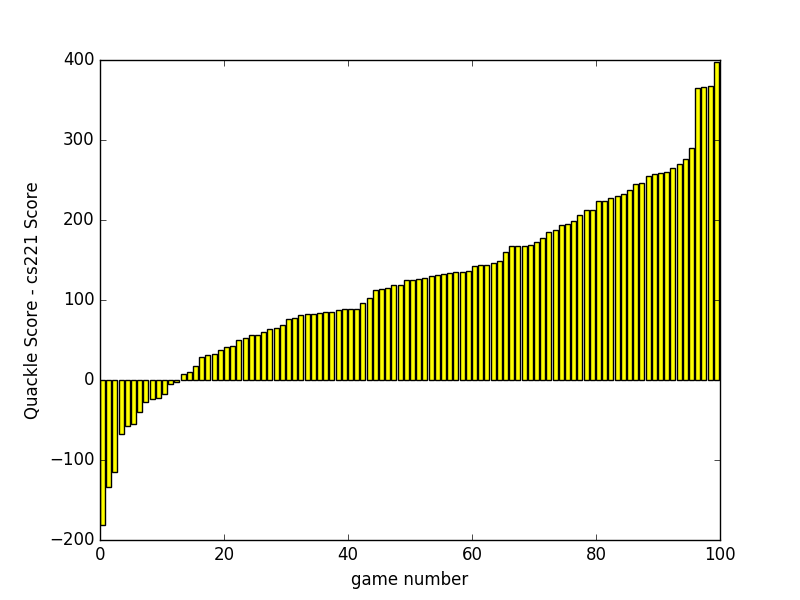
\includegraphics[scale=0.4]{../images/quacklegame_rackH_100}\\
   \caption{\footnotesize{Quackle vs CS221 w/ Rack Heuristics}}
  \endminipage{}
  \minipage{0.5\textwidth}
    \centering
  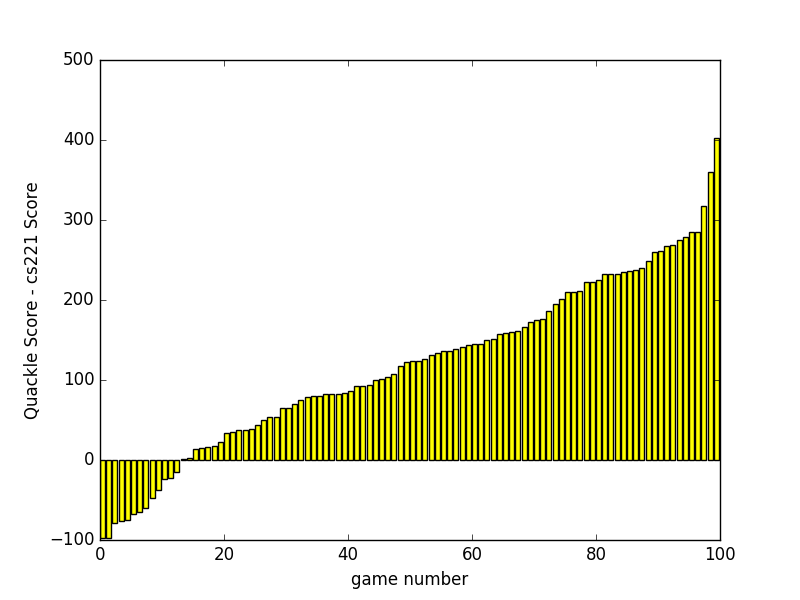
\includegraphics[scale=0.4]{../images/quacklegame_MC_100}
  \caption{\footnotesize{Quackle vs CS221 w/ Monte Carlo}}
  \endminipage
  \minipage{0.5\textwidth}
      \centering
  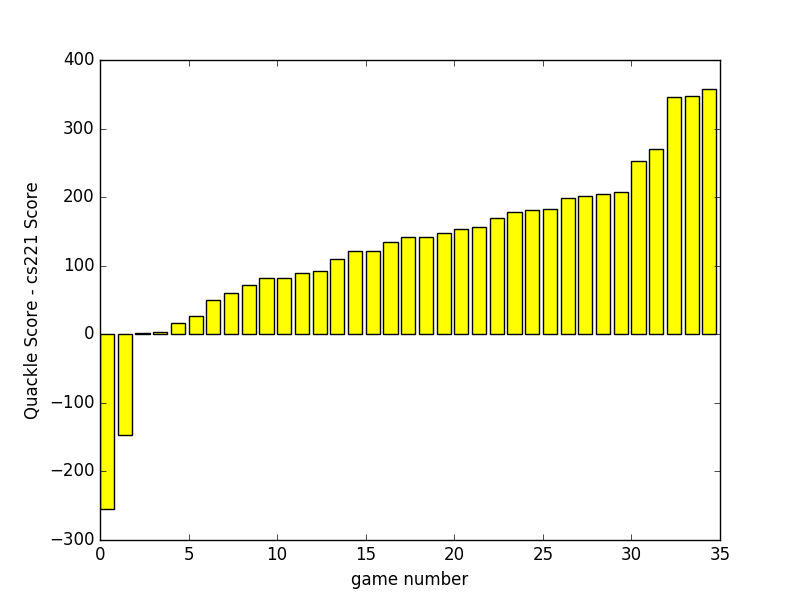
\includegraphics[scale=0.39]{../images/quacklegame_MC-RH_35}\\
   \caption{\footnotesize{Quackle vs CS221 with Monte Carlo and Rack
       Heuristics*}}
  \endminipage{}
\end{figure}

We were disappointed to see that the additional features like rack
heuristics and Monte Carlo didn't make a big difference in game
outcomes, at least while playing Quackle. We suspect that the gains
given by rack heuristics and Monte Carlo are only noticeable when two
AIs already perform comparably. The results of our selfplay games in
Table 2 support this, as we win against our own AI a statistically
significant amount more--a 62\% win rate compared to roughly 50-50 for
the control set.  

The rack heuristics perform similarly to the control. This is not
surprising considering our weight vectors though (which can be found
at the top of util.py). The weight for the raw score multiple orders
of magnitude higher than any other feature. This means that the moves
selected in the vanilla case and the rack heuristic case will not
often differ. However, in the rack heuristic + Monte Carlo case the
Monte Carlo score is only one order of magnitude smaller than the raw
score, which means that the Monte Carlo score non-trivially impacts
which move is ultimately selected. This is evidenced by the increased
win rate of 53\%. Unfortunately the weight vector used on this dataset
had a limited SGD run (50 iterations instead of 100). Also, since
Monte Carlo games take 10x longer to play, we needed to terminate the
data collection before it reached 100 games. We suspect that if we had
more time the results would be even better.


\begin{table}[h!]
  \centering
  \begin{tabular}{c|l|l|l|l|l|l}
    \textbf{} & \textbf{win rate} & \textbf{mean} & \textbf{opp mean} & \textbf{mean delta} &  \textbf{2x loss rate} & \textbf{max win ratio} \\\hline
  \textbf{control}   & 47\% & 354.24 & 359.25 & -5.01  & 0\%  & 1.811\\
  \textbf{RH}        & 48\% & 351.59 & 353.81 & -2.22  & 0\%  & 1.509\\
  \textbf{MC*}       & 62\% & 361.55 & 340.56 & 20.98  & 0\%  & 1.41 \\
  \textbf{MC w/ RH*} & 53\% & 364.62 & 347.07 & 17.54  & 0\%  & 1.33 \\
\end{tabular}
  \caption{Statistics of our AI playing against itself for 300
    games. Control is the vanilla variant playing against itself, all
    other rows are variations playing against vanilla. For description
    of columns, see caption for Table 1.}
\end{table}

One particular challenge to improving our performance was the long
development cycle. For example, after adding or removing features to
the feature extractor we need to re-run SGD and then re-run all
datasets that depend on a weight vector. This is very time consuming,
especially when we include Monte Carlo simulation, so we could only do
a limited amount of algorithmic experimentation.

Finally, we suspect that a large part of the gap is simplifications we
made to edge cases in gameplay. As mentioned earlier, we do not adapt
our strategy for the end game. We also do not do detailed analysis for
tile exchanges. We only exchange tiles if the Move Generator returns
empty, and we do not strategize which tiles to exchange from our
rack. Our wilcard behavior is also simplified--we simply choose a
vowel if our rack currently has none, otherwise we choose a tile
randomly. This is because a blank tile greatly increases the number of
possible moves and non-trivially modifying the existing search
algorithm.

Anecdotally, the AI does very well against average humans (the authors
and their friends), even if it probably won't beat a world champion.

\section*{Conclusion}
Considering that we are both new to AI and had only 6 weeks to work on
this project part-time, we are pretty happy that we managed to beat
the research-grade Quackle AI 13\% of the time.

Neither of the authors will be playing Scrabble again anytime soon.

\clearpage
\begin{center}
 \section*{Code Appendix}
\end{center}
Contents of scrabble folder:
\begin{itemize}
\setlength\itemsep{-0.22em}
\item agent.py: AI to choose an optimal move
\item autorun.py: quackle vs CS221 AI mode
\item brain.py: the Appel-Jacobsen move generator + Monte Carlo simulation
\item baseline.py: baseline implementation from proposal
\item board.py: the Scrabble board object 
\item boardTests.py: unit tests for board functionality
\item brainTests.py: unit tests for move generator
\item images/: images for our progress and final reports
\item letterbag.py: the object that holds Scrabble tiles
\item oracle.py: our oracle implementation
\item pdfs/: pdfs of our proposal, progress, and poster
\item pygtrie: the Google trie implementation we use for move generation
\item results/: raw results, plots and statistics. Raw data stored and processed in plot.py
\item run.py: human vs AI mode
\item scrabblewords.txt: our Scrabble dictionary
\item selfrun.py: selfplay mode
\item sga.py: implements stochastic gradient ascent
\item treeBuilder.py: builds the trie from scrabblewords.txt
\item trie.p: trie pickle
\item util.py: utility functions and variables
\end{itemize}

Human mode runs by simply executing \verb|python run.py|. Selfplay
runs via\\ \verb|python selfplay.py -n <NUM_GAMES>|. To use
autorun.py, you need to build Quackle. Follow the README in the root
of the quackle folder to build, and then go to quackle/test and
run \verb|qmake test.pro && make|

This will create an executable called 'test' in quackle/test. We'll be
running the test program with these options:
\verb|./test --repetitions=N lexicon=cs221 --mode=cs221|

This tells the quackle test harness to run N games in cs221 mode with
the cs221 lexicon. The code for cs221 mode is mainly defined in the
function selfPlayCS221Game() inside test/testharness.cpp.

The Python half is in scrabble/autorun.py. It interfaces with the
quackle AI via text files in quackle/test. Quackle's data is written
to quackle/test/quacklegame-n.gcg, which autorun.py reads and
parses. After parsing and committing the quackle move, our AI
calculates its own move, commits it, and writes it to the file
test/quackle/cs221game-n.

To run Quackle vs. CS221:

\verb|python autorun.py -n <NUM_GAMES> -p <PATH_TO_QUACKLE_TEST>|

Optionally, add a \texttt{-s} flag to suppress ASCII-board output,
useful when running large batches.

\vspace{ 8cm }
\clearpage
\begin{center}
{\Large References}
\end{center} 
A.W. Appel, G.J. Jacobson, The world’s fastest Scrabble program, Comm. ACM 31 (5) (1988) 572–578, 585. \\
Mark Richards and Eyal Amir. Opponent Modeling in Scrabble. IJCAI-07., 1482–1487, 2007. \\
Stuart Russell and Peter Norvig. Artificial Intelligence: A Modern Approach. Prentice-Hall,
Englewood Cliffs, NJ, 2nd edition edition, 2003 \\
Brian Sheppard. World-championship caliber Scrabble. Artif. Intell., 134:241–245, 2002. \\
J. Katz-Brown, J. O'Laughlin, J. Fultz, M. Liberty, A. Buddhdev, Quackle,\\ http://people.csail.mit.edu/jasonkb/quackle/
\end{document}
